% =====================================================================
%  CHAPITRE 3 -- partie c : section 3.4 (cas appliques) et 3.5 (synthese)
% =====================================================================

% ---------------------------------------------------------------- 35
\begin{frame}{Section 3.4 --- Cas appliqué 1 : Gamma-Poisson (taux d'accidents)}
\begin{columns}[t]
\begin{column}{0.51\textwidth}
\begin{ebox}[Énoncé]
Un site industriel a enregistré
\[
y = (12,\ 9,\ 14,\ 11,\ 13,\ 8) \quad\text{accidents sur 6 mois},
\]
soit $s = 67$ accidents au total. On modélise
\[
y_i \given \lambda \sim \mathcal{P}(\lambda),
\qquad
\lambda \sim \mathrm{Gamma}(\alpha_0\,; \beta_0).
\]
Par conjugaison :
\[
\lambda \given y \sim \mathrm{Gamma}\big(\alpha_0 + 67\,;\, \beta_0 + 6\big).
\]
\end{ebox}
\end{column}
\begin{column}{0.47\textwidth}
\begin{kbox}[Trois questions décisives]
\begin{enumerate}
  \item Quelle est le taux mensuel d'accidents, \textbf{avec son incertitude} ?
  \item Le seuil réglementaire de $12$ accidents par mois est-il franchi ?
  \item Que devient la réponse si l'on change de prior --- autrement dit,
        quelle part de la conclusion vient des \textbf{données} ?
\end{enumerate}
\vspace{1mm}
\footnotesize Le MLE vaut $s/n = 67/6 = 11{,}167$ : il répond à (1) par un point,
et ne répond pas du tout à (2) et (3).
\end{kbox}
\end{column}
\end{columns}
\vspace{1mm}
\begin{tcolorbox}[colback=byCyan!8,colframe=byCyan,arc=2mm,width=.95\textwidth]
\centering\small
\textbf{La question du prior} : six mois d'historique, c'est peu. Trois priors
seront comparés --- et la comparaison \emph{est} le résultat, pas un préliminaire.
\end{tcolorbox}
\end{frame}

% ---------------------------------------------------------------- 36
% [rogna]
% [rogna]
% [rogna]
\begin{frame}{Gamma-Poisson : le prior change-t-il la conclusion ?}
\begin{center}
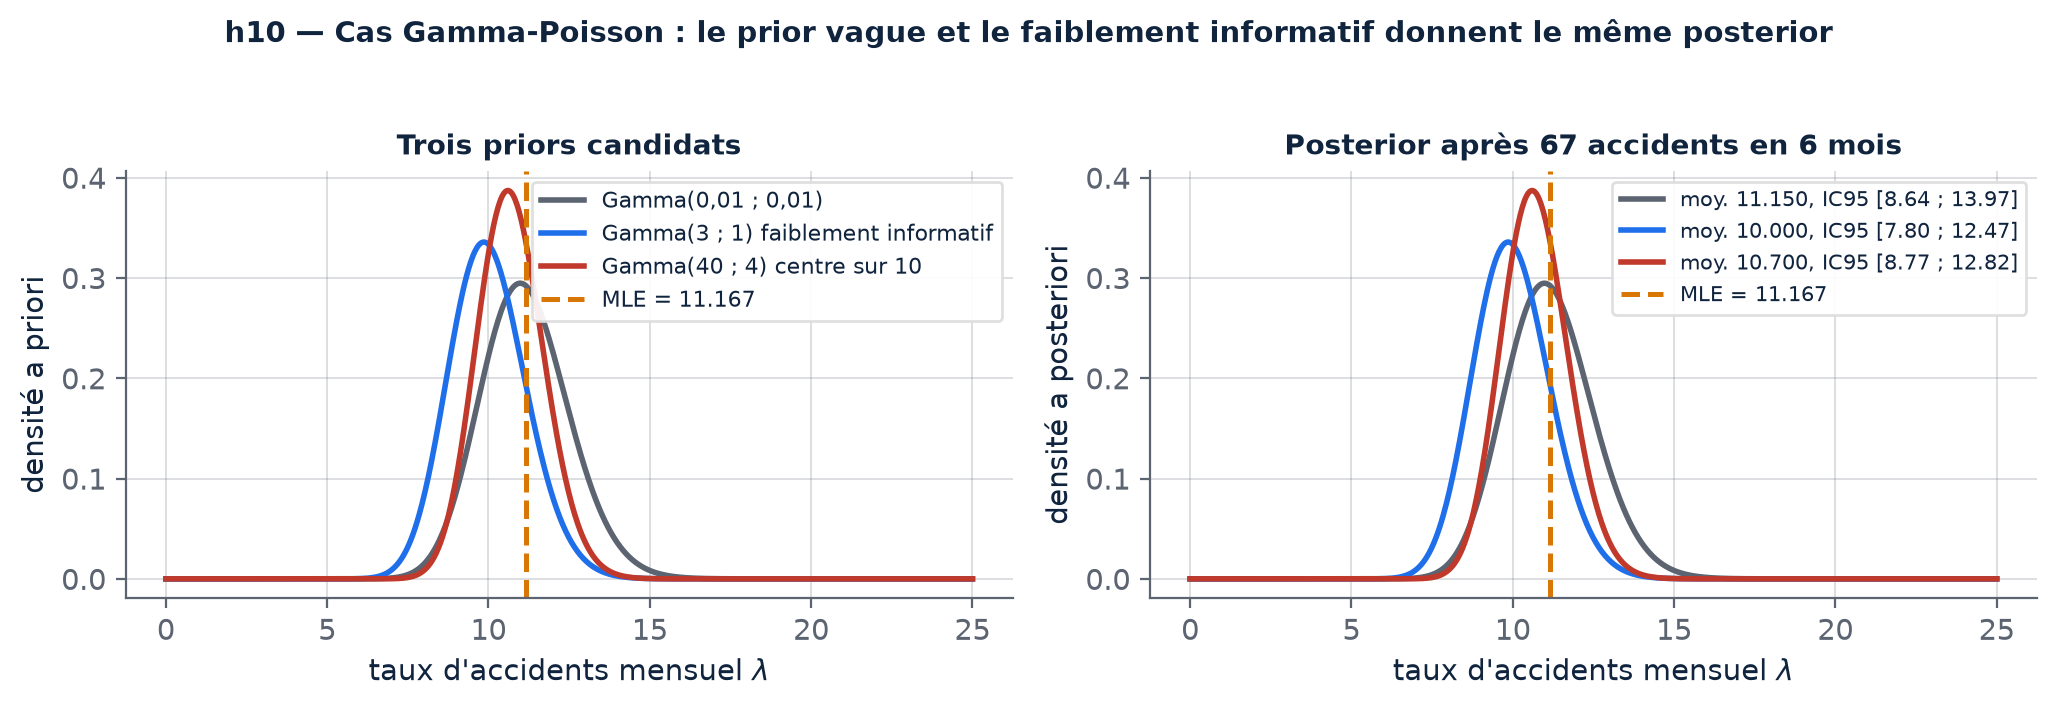
\includegraphics[width=.88\textwidth]{h10_gamma_poisson.png}
\end{center}
\end{frame}

\begin{frame}{Gamma-Poisson : le prior change-t-il la conclusion ?}
\small
\begin{solbox}[Posterior et crédibilité, calculés]
\footnotesize
\centering
\resizebox{\ifdim\width>\linewidth\linewidth\else\width\fi}{!}{%
\begin{tabular}{@{}lccc@{}}
\toprule
Prior & moyenne & IC $95\,\%$ & largeur \\
\midrule
Gamma$(0{,}01\,;0{,}01)$ & $11{,}150$ & $[8{,}64\,;13{,}97]$ & $5{,}332$ \\
Gamma$(3\,;1)$ & $10{,}000$ & $[7{,}80\,;12{,}48]$ & $4{,}679$ \\
Gamma$(40\,;4)$ & $10{,}700$ & $[8{,}77\,;12{,}82]$ & $4{,}052$ \\
\midrule
\multicolumn{4}{@{}l@{}}{\textbf{MLE} : $11{,}167$} \\
\bottomrule
\end{tabular}}
\vspace{1.5mm}

$P(\lambda > 12 \given y)$ : $0{,}258$ (prior vague) contre $0{,}107$ (prior fort).
\end{solbox}
\vspace{1mm}
\begin{columns}[t]
\begin{column}{0.49\textwidth}
\begin{kbox}[Leçon 1 : les données dominent]
Le prior vague et le prior faiblement informatif donnent la \emph{même} réponse à
$1\,\%$ près : avec $67$ événements, la vraisemblance écrase toute croyance molle.
\end{kbox}
\end{column}
\begin{column}{0.49\textwidth}
\begin{kbox}[Leçon 2 : un prior fort engage]
Avec Gamma$(40\,;4)$ --- un site \emph{a priori} sûr --- la probabilité de franchir
le seuil tombe de $26\,\%$ à $11\,\%$. Un prior fort doit être \textbf{documenté}.
\end{kbox}
\end{column}
\end{columns}
\end{frame}

% ---------------------------------------------------------------- 37
\begin{frame}{Section 3.4 --- Cas appliqué 2 : Normal-Normal (mesures répétées)}
\small
\vspace{-1.5mm}
\begin{columns}[t]
\begin{column}{0.53\textwidth}
\begin{ebox}[Énoncé : pesée d'un lot de poudre]
Sept mesures ont été faites sur le même échantillon :
\[
y = (112,\ 121,\ 108,\ 117,\ 126,\ 115,\ 119)\ \mathrm{g},\qquad
\bar y = 116{,}857 .
\]
On connaît le bruit de la balance : $\sigma = 8$ g. Le vrai poids moyen suit un
prior $\mathcal{N}(\mu_0, \tau_0^2)$ avec $\mu_0 = 100$, $\tau_0 = 15$.
\end{ebox}
\begin{kbox}[Conjugaison par les \textbf{précisions}]
\vspace{-1mm}
\[
\frac{1}{\sigma_{\text{post}}^2} = \frac{1}{\tau_0^2} + \frac{n}{\sigma^2},
\qquad
\mu_{\text{post}} = \sigma_{\text{post}}^2\left(\frac{\mu_0}{\tau_0^2} + \frac{n\bar y}{\sigma^2}\right)
\]
\end{kbox}
\end{column}
\begin{column}{0.45\textwidth}
\begin{solbox}[Calcul exécuté]
{\footnotesize
$\frac{1}{\sigma_{\text{post}}^2} = \frac{1}{225} + \frac{7}{64} = 0{,}11382$
\[
\Rightarrow\; \sigma_{\text{post}} = 2{,}964, \quad \mu_{\text{post}} = 116{,}199
\]
crédibilité $95\,\%$ : $[110{,}39\,;122{,}01]$
}
\vspace{1mm}
\footnotesize L'écart-type a posteriori ($2{,}96$) est à peine inférieur à celui
de la moyenne des mesures $\sigma/\sqrt n = 3{,}02$ : la réduction vaut
$1{,}97\,\%$ seulement. Le prior, ici, \textbf{n'apporte presque rien}.
\end{solbox}
\end{column}
\end{columns}
\vspace{1mm}
\begin{tcolorbox}[colback=byLight,colframe=byGrey!55,arc=2mm,width=.95\textwidth]
\centering\small
\textbf{Le réflexe à acquérir} : comparer $\sigma_{\text{post}}$ à $\sigma/\sqrt n$.
Si le prior améliorait vraiment, on verrait $\sigma_{\text{post}} \ll \sigma/\sqrt n$.
Dans cet exemple, $7$ mesures valent plus que l'expert.
\end{tcolorbox}
\end{frame}

% ---------------------------------------------------------------- 38
\begin{frame}{Normal-Normal : mise à jour et prédiction de la prochaine mesure}
\small
\vspace{-2mm}
\begin{center}
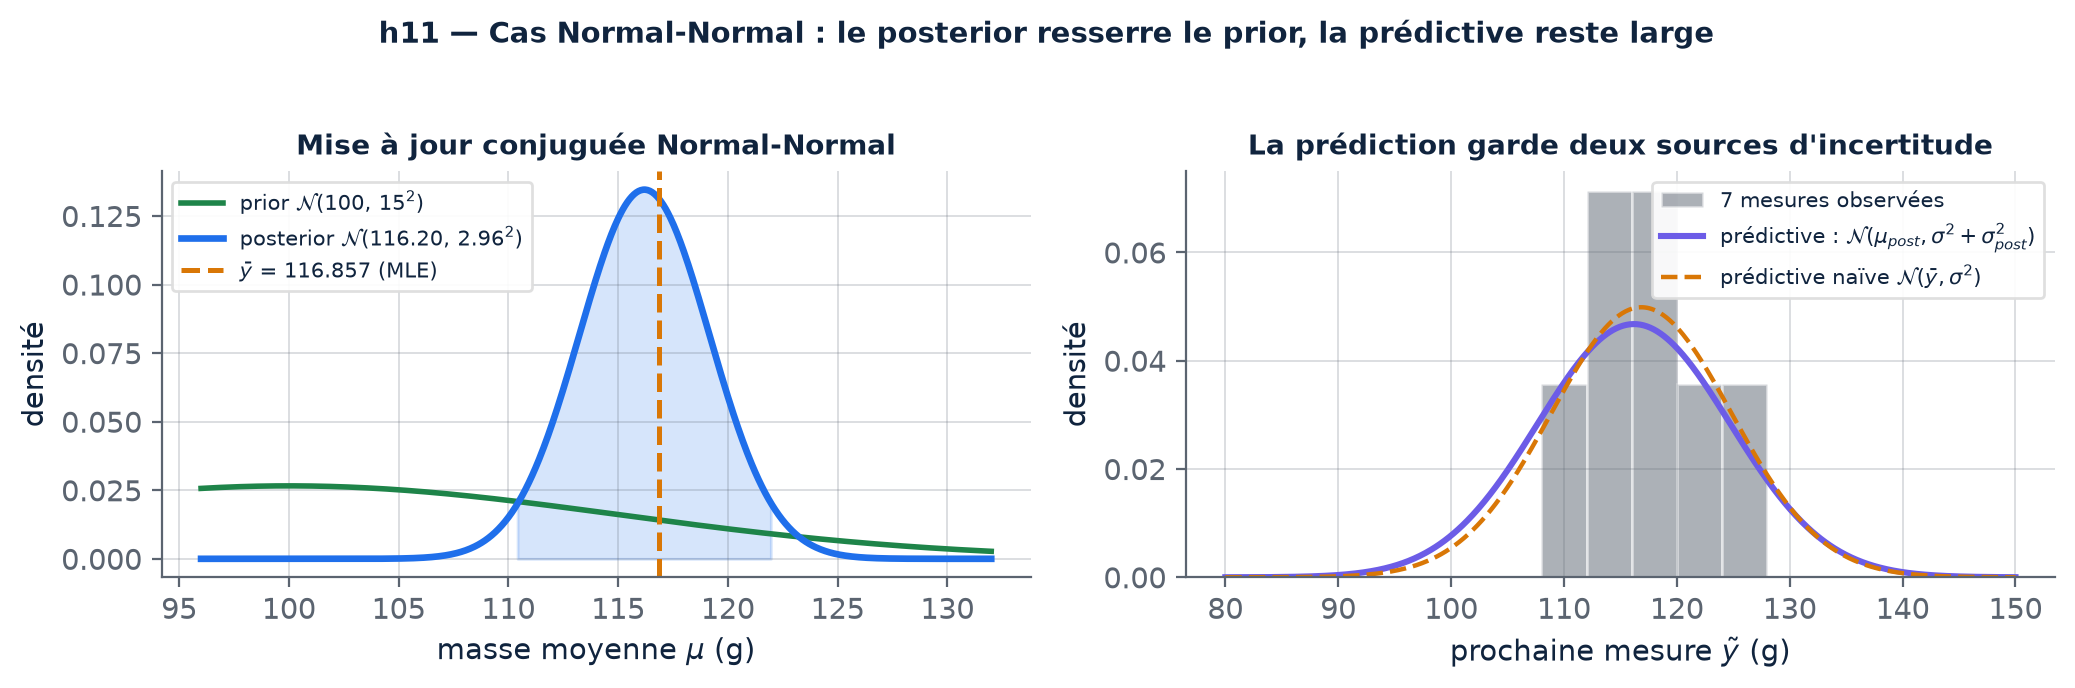
\includegraphics[width=.74\textwidth]{h11_normal_normal.png}
\end{center}
\vspace{-1.5mm}
\begin{columns}[t]
\begin{column}{0.56\textwidth}
\begin{ebox}[Les deux panneaux, lus dans le bon ordre]
À gauche : le prior $\mathcal{N}(100, 15^2)$ se resserre en
$\mathcal{N}(116{,}20\,; 2{,}96^2)$ autour de $\bar y = 116{,}86$.
À droite : la prédiction de la \emph{prochaine} mesure garde l'incertitude de
mesure, donc elle reste large.
\end{ebox}
\end{column}
\begin{column}{0.42\textwidth}
\begin{solbox}[Écart-type prédictif]
{\footnotesize
\[
\sigma_{\text{pred}} = \sqrt{\sigma^2 + \sigma_{\text{post}}^2} = \sqrt{64 + 8{,}79}
\]
\[
= \mathbf{8{,}53}
\]
}
Intervalle prédictif $95\,\%$ : $[99{,}48\,;132{,}92]$, de largeur $33{,}44$
--- contre $31{,}36$ pour l'approche naïve. \textbf{La différence est le prix
de l'honnêteté.}
\end{solbox}
\end{column}
\end{columns}
\end{frame}

% ---------------------------------------------------------------- 39
\begin{frame}[fragile]{Régression linéaire bayésienne complète en PyMC}
\footnotesize
\vspace{-2.5mm}
\begin{codebox}[Modèle, échantillonnage et résumé --- code réellement exécuté]
\begin{lstlisting}
import numpy as np, pymc as pm, arviz as az
n = 25
x = np.sort(rng.uniform(0.2, 5.0, n))
y = 2.0 + 1.5 * x + rng.normal(0.0, 0.9, n)   # verite : a=2, b=1.5, s=0.9
with pm.Model() as mreg:
    alpha = pm.Normal("alpha", mu=0.0, sigma=5.0)   # priors faiblement informatifs
    beta  = pm.Normal("beta",  mu=0.0, sigma=5.0)
    sigma = pm.HalfNormal("sigma", sigma=2.0)
    mu    = alpha + beta * x
    pm.Normal("y", mu=mu, sigma=sigma, observed=y)  # vraisemblance = modele lineaire
    idata = pm.sample(draws=1000, tune=600, chains=2, cores=1, random_seed=3)
print(az.summary(idata, var_names=["alpha", "beta", "sigma"]))  # R-hat, ESS, moyennes
\end{lstlisting}
\end{codebox}
\vspace{0.5mm}
\begin{columns}[t]
\begin{column}{0.56\textwidth}
\begin{kbox}[Pourquoi ces priors ?]
$\mathcal{N}(0, 5^2)$ laisse $\alpha$ et $\beta$ parcourir $\pm 10$ : c'est
\textbf{informations nulles}. Un $\mathcal{HalfNormal}(2)$ sur $\sigma$ interdit
les variabilités absurdes sans fixer l'échelle : le prior doit se \emph{voir}
sans se \emph{sentir}.
\end{kbox}
\end{column}
\begin{column}{0.42\textwidth}
\begin{solbox}[Coût réel de l'exécution]
\begin{itemize}
  \item $2$ chaînes $\times$ $1\,000$ tirages $= 2\,000$ échantillons, en $348$ s
        sur CPU (sans compilateur C ni GPU) ;
  \item $\hat R$ max $= 1{,}0034$, ESS min $= 908$, $0$ divergence.
\end{itemize}
\end{solbox}
\end{column}
\end{columns}
\end{frame}

% ---------------------------------------------------------------- 40
\begin{frame}{Posterior des coefficients : nuage, bandes et posterior joint}
\small
\vspace{-1.5mm}
\begin{center}
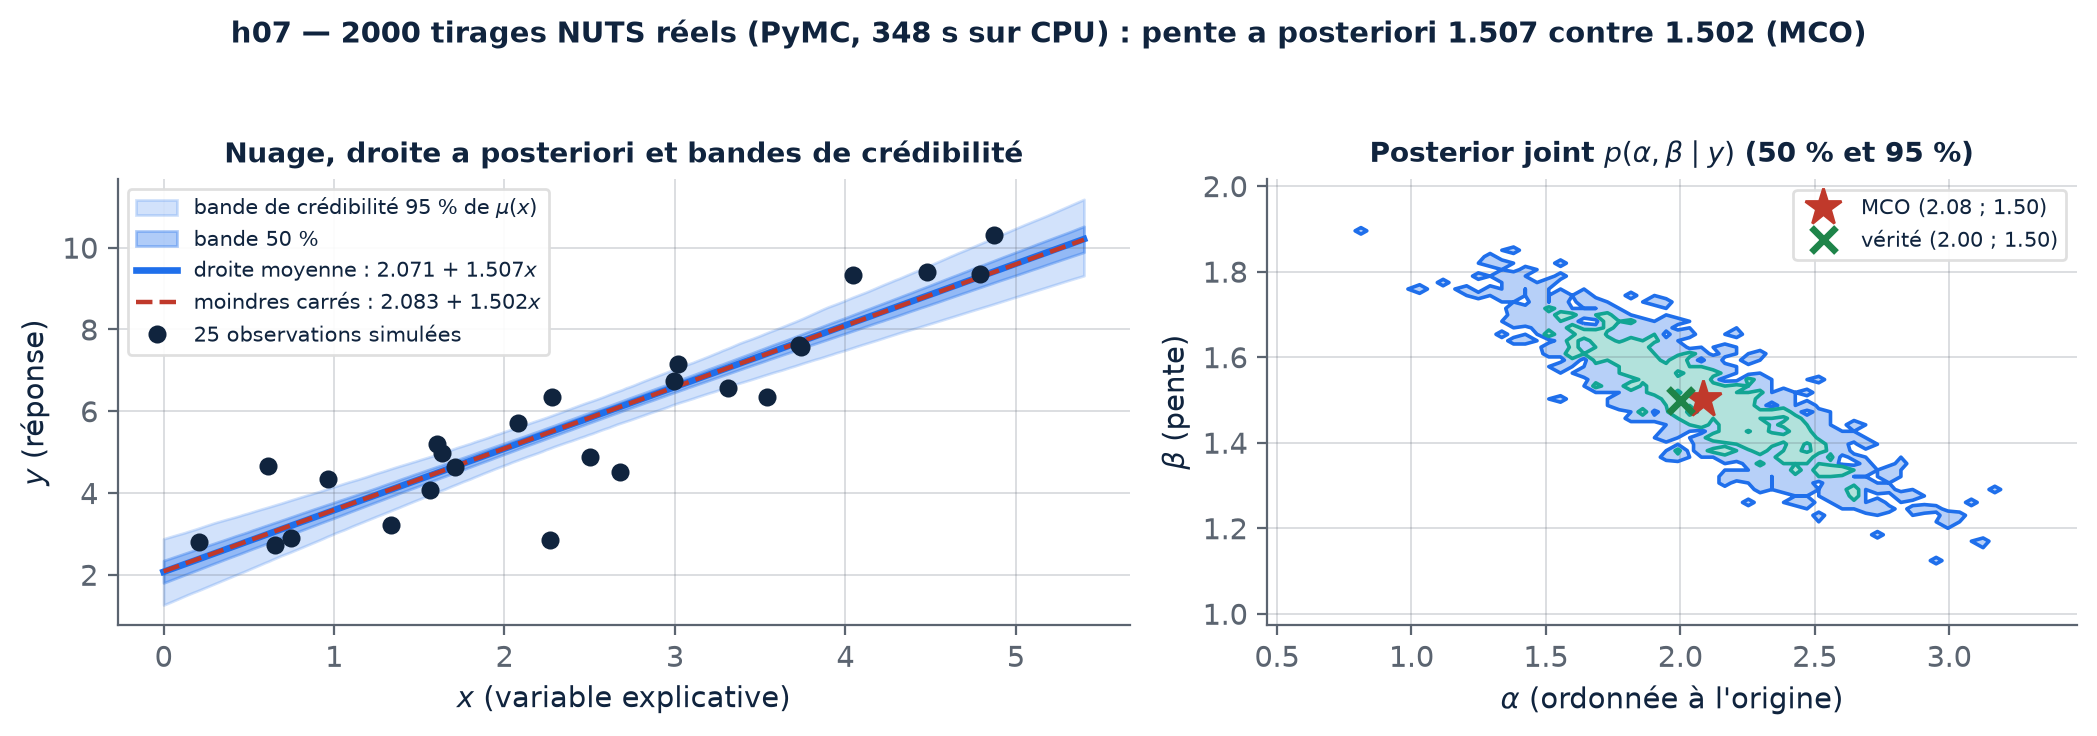
\includegraphics[width=.76\textwidth]{h07_regression_bayesienne.png}
\end{center}
\vspace{-1.5mm}
\begin{columns}[t]
\begin{column}{0.54\textwidth}
\begin{ebox}[Trois colonnes, trois lectures]
À gauche : nuage, droite moyenne et bandes de crédibilité $50\,\%$ et $95\,\%$
de $\mu(x)$. Au centre : le posterior \textbf{joint} $p(\alpha, \beta \given y)$.
À droite : la pente, indiscernable des MCO.
\end{ebox}
\end{column}
\begin{column}{0.44\textwidth}
\begin{solbox}[Chiffres de l'échantillonnage]
\resizebox{\ifdim\width>\linewidth\linewidth\else\width\fi}{!}{%
\begin{tabular}{@{}lccc@{}}
\toprule
Paramètre & MCO & Bayes & vérité \\
\midrule
$\alpha$ & $2{,}083$ & $2{,}071$ & $2{,}00$ \\
$\beta$  & $1{,}502$ & $1{,}507$ & $1{,}50$ \\
$\sigma$ & ---      & $0{,}995$ & $0{,}90$ \\
\bottomrule
\end{tabular}}
\vspace{1.5mm}

HDI $95\,\%$ de $\beta$ : $[1{,}236\,;1{,}797]$ (contient $1{,}5$) ;
$P(\beta > 1 \given y) = 0{,}9995$.
\end{solbox}
\end{column}
\end{columns}
\end{frame}

% ---------------------------------------------------------------- 41
\begin{frame}{Diagnostics MCMC réels : peut-on croire ces tirages ?}
\small
\vspace{-1.5mm}
\begin{center}
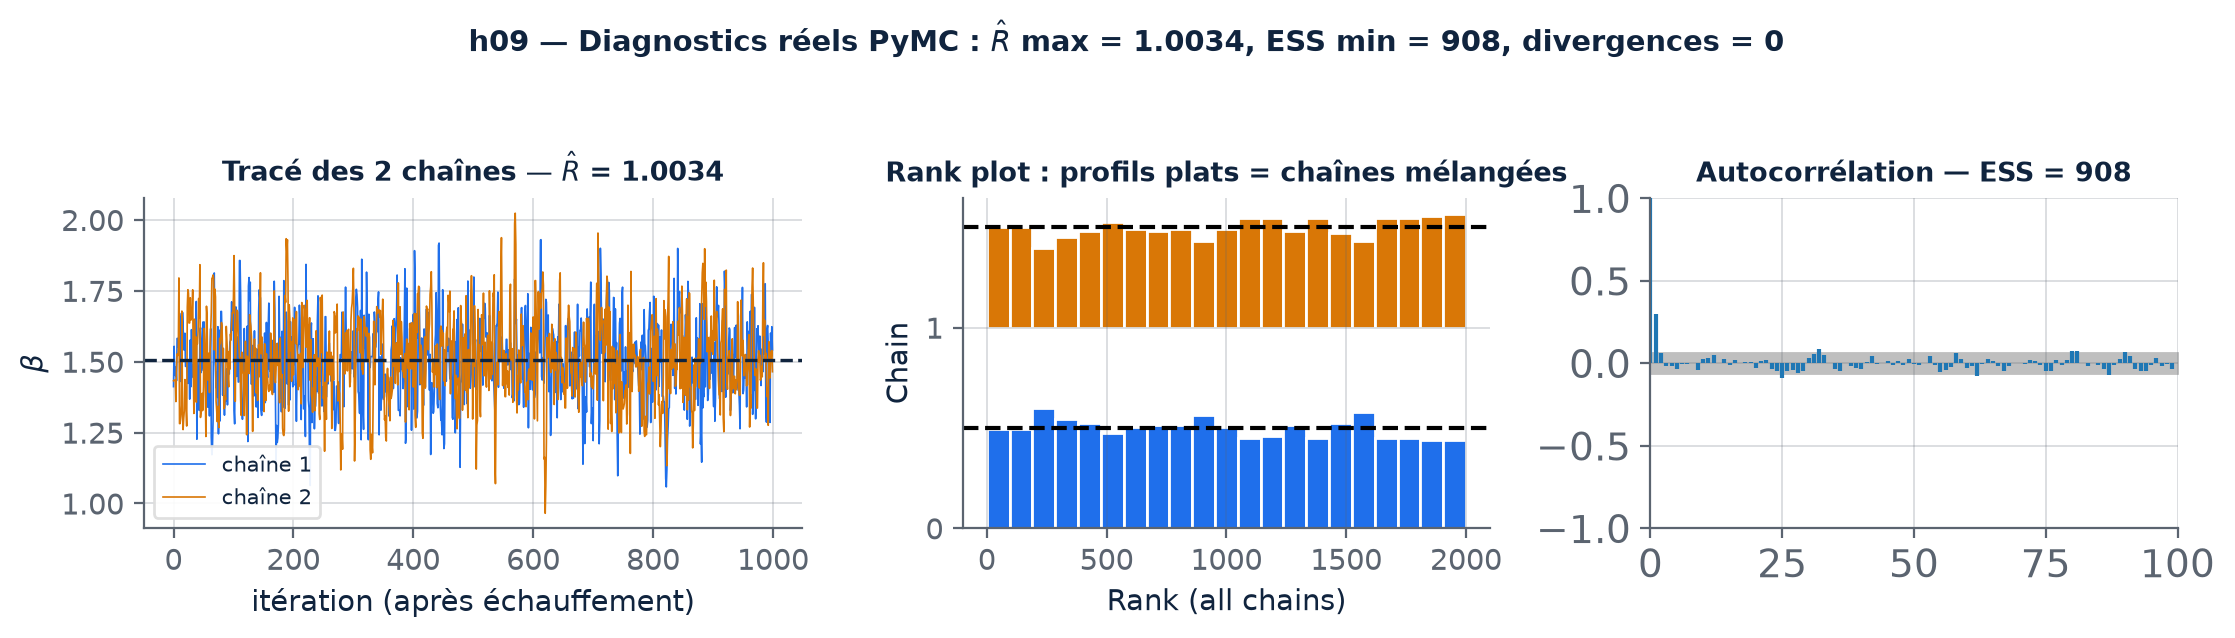
\includegraphics[width=.84\textwidth]{h09_pymc_trace.png}
\end{center}
\vspace{-1.5mm}
\begin{columns}[t]
\begin{column}{0.55\textwidth}
\begin{ebox}[Le trio de contrôle, valeurs lues sur cette exécution]
\begin{tabular}{@{}lccc@{}}
\toprule
Paramètre & $\hat R$ & ESS & divergences \\
\midrule
$\alpha$ & $1{,}0034$ & $918{,}0$ & $0$ \\
$\beta$  & $1{,}0024$ & $907{,}9$ & $0$ \\
$\sigma$ & $1{,}0022$ & $1\,043{,}0$ & $0$ \\
\bottomrule
\end{tabular}
\vspace{1mm}
\footnotesize $\hat R$ proche de $1$ et ESS élevé : les deux chaînes explorent la
même loi. Un tracé « en chenille » sans dérive et un rank plot plat confirment
visuellement ce que les nombres disent.
\end{ebox}
\end{column}
\begin{column}{0.43\textwidth}
\begin{kbox}[Seuils usuels à retenir]
\begin{itemize}
  \item $\hat R < 1{,}01$ (idéalement $< 1{,}005$) ;
  \item $\mathrm{ESS} > 400$ par paramètre ;
  \item $0$ divergence, $0$ message d'avertissement ;
  \item sinon : augmenter \py{tune}, reparamétrer (centrer $x$), ou changer de prior.
\end{itemize}
\end{kbox}
\end{column}
\end{columns}
\end{frame}

% ---------------------------------------------------------------- 42
\begin{frame}{Densités marginales et deux notions d'intervalle}
\small
\vspace{-2mm}
\begin{center}
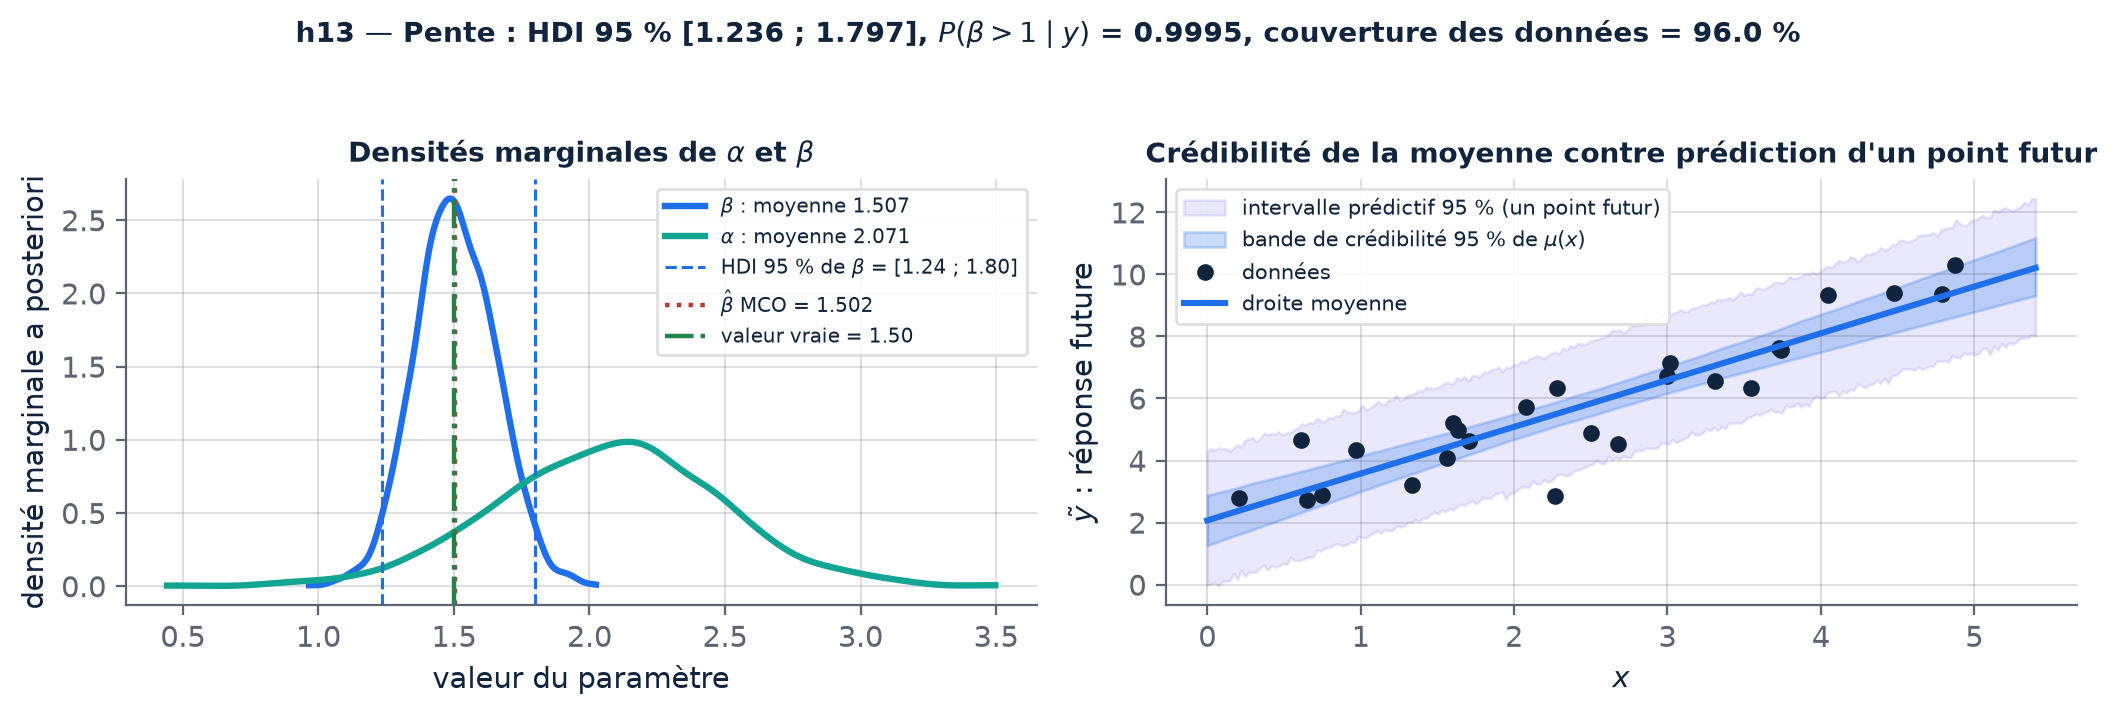
\includegraphics[width=.72\textwidth]{h13_regression_marginales.png}
\end{center}
\vspace{-1.5mm}
\begin{columns}[t]
\begin{column}{0.55\textwidth}
\begin{ebox}[Ce que la figure sépare nettement]
À gauche : les densités marginales de $\alpha$ et $\beta$ ; l'HDI $95\,\%$ de
$\beta$, $[1{,}236\,;1{,}797]$, \textbf{couvre} la valeur vraie $1{,}5$, et la
pente MCO ($1{,}502$) tombe au centre.
À droite : la \textbf{bande de crédibilité} de $\mu(x)$ (étroite) et
l'\textbf{intervalle prédictif} d'une observation future (large) --- deux
questions différentes.
\end{ebox}
\end{column}
\begin{column}{0.43\textwidth}
\begin{solbox}[Contrôle prédictif exécuté]
Sur les $25$ observations, $96\,\%$ (soit $24/25$) tombent dans l'intervalle
prédictif à $95\,\%$ : conforme à l'attendu, le modèle reproduit les données
observées.
\end{solbox}
\begin{kbox}[Phrase à écrire dans un rapport]
« La pente vaut $1{,}51$, intervalle de crédibilité $95\,\%$
$[1{,}24\,;1{,}80]$ » : jamais « $\pm$ ».
\end{kbox}
\end{column}
\end{columns}
\end{frame}

% ---------------------------------------------------------------- 43
\begin{frame}{Bande de crédibilité contre intervalle de prédiction}
\begin{columns}[t]
\begin{column}{0.49\textwidth}
\begin{tcolorbox}[enhanced,colback=byBlue!6,colframe=byBlue,arc=2mm,
   title={\bfseries\color{white} Bande de crédibilité de $\mu(x)$},colbacktitle=byBlue,
   attach boxed title to top left={xshift=3mm,yshift=-2mm},
   boxed title style={arc=1mm,boxrule=0pt}]
\begin{itemize}
  \item Question : « où se situe la \textbf{moyenne} du processus ? »
  \item Se resserre comme $1/\sqrt n$ et peut devenir très étroite.
  \item Utile pour comparer des groupes, tester un effet, communiquer une
        estimation.
\end{itemize}
\end{tcolorbox}
\end{column}
\begin{column}{0.49\textwidth}
\begin{tcolorbox}[enhanced,colback=byPurple!7,colframe=byPurple,arc=2mm,
   title={\bfseries\color{white} Intervalle de prédiction de $\tilde y$},colbacktitle=byPurple,
   attach boxed title to top left={xshift=3mm,yshift=-2mm},
   boxed title style={arc=1mm,boxrule=0pt}]
\begin{itemize}
  \item Question : « quelle valeur \textbf{individuelle} vais-je observer ? »
  \item Ne descend \textbf{jamais} sous le bruit intrinsèque $\sigma$ :
        largeur $\geq 2 \times 1{,}96\,\sigma$.
  \item Utile pour dimensionner, garantir, alerter.
\end{itemize}
\end{tcolorbox}
\end{column}
\end{columns}
\vspace{1mm}
\begin{wbox}[La confusion la plus coûteuse en pratique]
\small Annoncer la bande de crédibilité de la \emph{moyenne} comme une garantie sur
les \emph{individus}. Sur l'exemple de la balance : la moyenne est connue à
$\pm 5{,}8$ g ($95\,\%$), mais chaque pesée future peut s'écarter de $\pm 16{,}7$ g.
Confondre les deux, c'est promettre au client une tolérance
\textbf{deux fois} trop serrée.
\end{wbox}
\end{frame}

% ---------------------------------------------------------------- 44
% [split]
\begin{frame}{Risque MSE : estimateur bayésien contre maximum de vraisemblance}
\begin{center}
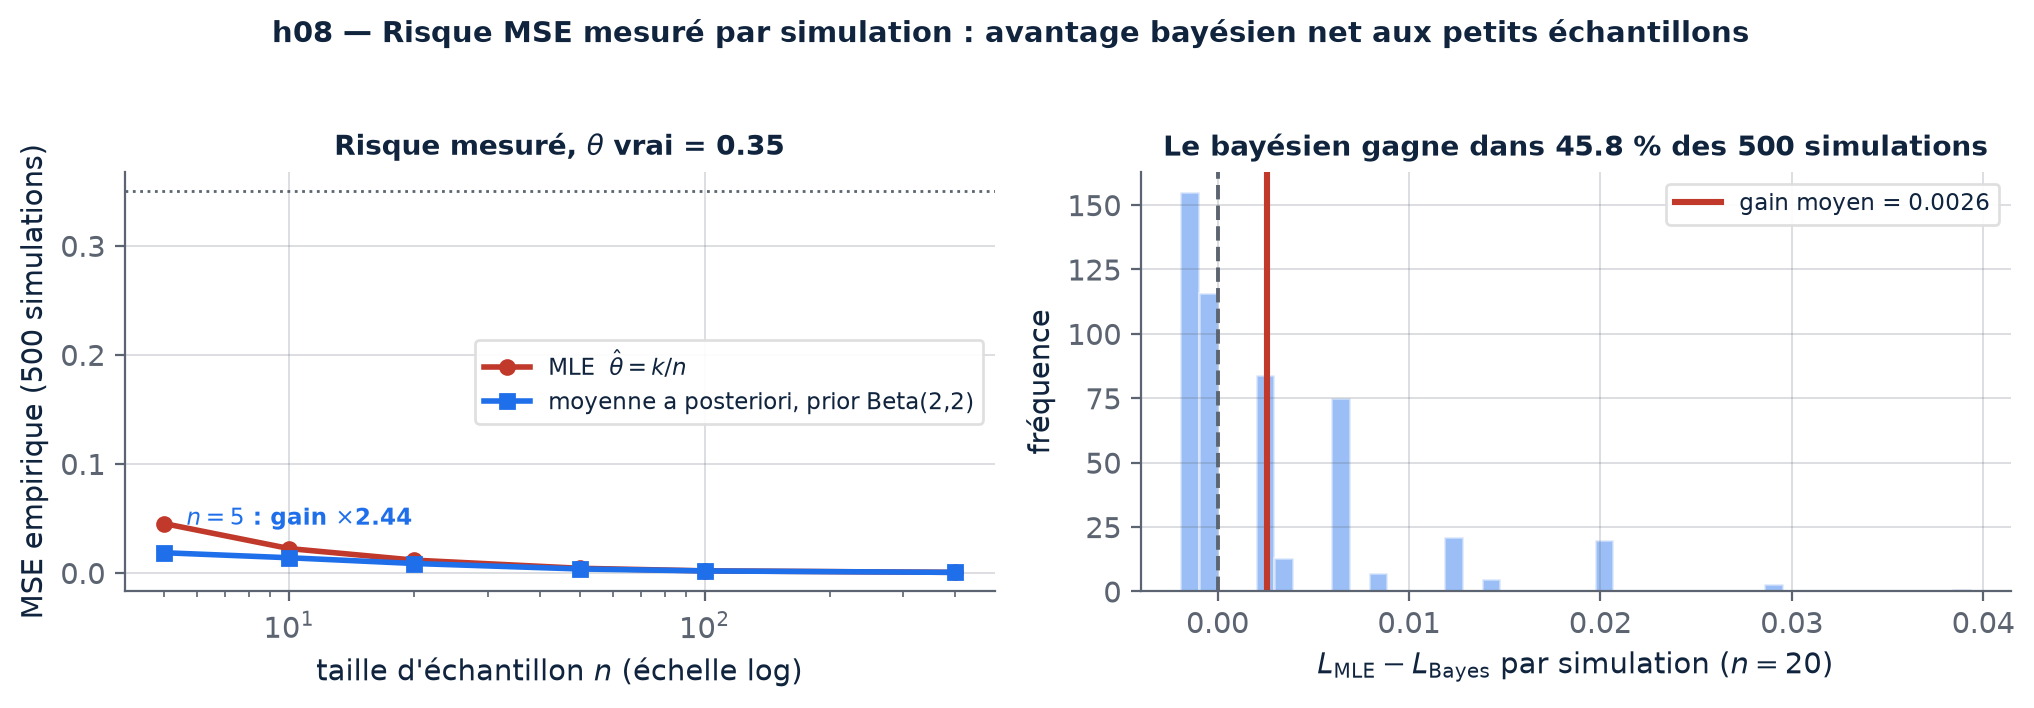
\includegraphics[width=.86\textwidth]{h08_mse_bayes_vs_mle.png}
\end{center}
\end{frame}

% [split]
\begin{frame}{Risque MSE : estimateur bayésien contre maximum de vraisemblance}
\small
\vspace{-2mm}

\vspace{-1.5mm}
\begin{columns}[t]
\begin{column}{0.56\textwidth}
\begin{ebox}[Protocole : 500 simulations réelles]
$\theta_{\text{vrai}} = 0{,}35$ ; pour chaque $n \in \{5, 10, 20, 50, 100, 400\}$,
on simule $500$ jeux de données, on calcule
$\hat\theta_{\text{MLE}} = k/n$ et
$\hat\theta_{\text{Bayes}} = (k+2)/(n+4)$ (prior Beta$(2,2)$), puis le MSE
empirique. Aucune formule asymptotique n'est invoquée : on \emph{mesure}.
\end{ebox}
\end{column}
\begin{column}{0.42\textwidth}
\begin{solbox}[Résultats mesurés]
\footnotesize
\resizebox{\ifdim\width>\linewidth\linewidth\else\width\fi}{!}{%
\begin{tabular}{@{}lccc@{}}
\toprule
$n$ & MSE MLE & MSE Bayes & rapport \\
\midrule
$5$ & $0{,}04526$ & $0{,}01853$ & $\mathbf{0{,}41}$ \\
$20$ & --- & --- & $0{,}74$ \\
$400$ & $0{,}000518$ & $0{,}000518$ & $1{,}00$ \\
\bottomrule
\end{tabular}}
\vspace{1.5mm}

Gain moyen à $n = 20$ : $0{,}00259$, positif dans $45{,}8\,\%$ des $500$ simulations.
\end{solbox}
\end{column}
\end{columns}
\vspace{1mm}
\begin{kbox}[Comment lire la variabilité du gain]
Le gain est positif \emph{en moyenne} mais pas à chaque tirage : un estimateur
rétréci peut perdre sur un échantillon particulier. C'est le prix de
l'amélioration en risque --- et la raison pour laquelle on recommande le bayésien
pour des \textbf{problèmes répétés}, pas pour un cas unique.
\end{kbox}
\end{frame}

% ---------------------------------------------------------------- 45
\begin{frame}{Atelier --- du modèle à la décision (TP noté, 30 min)}
\footnotesize
\vspace{-2mm}
\begin{abox}[Énoncé du TP]
On dispose d'un jeu de données réel (prix de logements, $n = 200$). On demande :
\begin{enumerate}
  \item Écrire le modèle de régression bayésien en PyMC (priors faiblement
        informatifs sur $\alpha$, $\beta$, $\sigma$).
  \item Échantillonner avec \py{pm.sample()} et vérifier $\hat R < 1{,}01$ et
        $\mathrm{ESS} > 400$.
  \item Produire le nuage + la droite a posteriori + les bandes $50\,\%$ et
        $95\,\%$.
  \item Rapporter l'effet mesuré : moyenne, HDI $95\,\%$, $P(\beta > 0 \given y)$.
  \item Conclure en \textbf{une phrase de décision} pour un agent immobilier :
        « chaque m\textsuperscript{2} supplémentaire vaut X, avec un intervalle
        de [\ldots] ».
\end{enumerate}
\end{abox}
\vspace{1mm}
\begin{columns}[t]
\begin{column}{0.49\textwidth}
\begin{kbox}[Grille d'évaluation]
4 pts modèle correct ; 2 pts diagnostics affichés ; 4 pts figure lisible avec
légende ; 6 pts interprétation (estimateur choisi et perte justifiée) ;
4 pts qualité du code (reproductible, \py{random_seed} fixé).
\end{kbox}
\end{column}
\begin{column}{0.49\textwidth}
\begin{qbox}[Question de contrôle]
Un étudiant annonce « $\beta = 1200$~euros/m\textsuperscript{2}, intervalle de
crédibilité $[900\,;1500]$ ». Que manque-t-il à cette phrase pour être
\emph{utilisable} ?
\vspace{1mm}

\textbf{Éléments attendus} : le niveau ($95\,\%$), le type d'intervalle (HDI ou
queues égales), et la précision que c'est l'effet sur la \emph{moyenne}, pas un
intervalle de prédiction pour un logement individuel.
\end{qbox}
\end{column}
\end{columns}
\end{frame}

% ---------------------------------------------------------------- 46
% [suite]
\begin{frame}{Section 3.5 --- Synthèse : du posterior à la décision, en un tableau}
\begin{center}
\small
\begin{tabular}{@{}p{3.3cm}p{3.4cm}p{4.4cm}p{3.2cm}@{}}
\toprule
\textbf{Besoin du commanditaire} & \textbf{Outil bayésien} & \textbf{Sortie chiffrée} & \textbf{Section} \\
\midrule
« Donnez-moi un chiffre » & moyenne / médiane / MAP &
$0{,}300$ / $0{,}286$ / $0{,}250$ sur Beta$(3,7)$ & 3.1 \\
\addlinespace
« Une fourchette crédible » & HDI $95\,\%$ &
$[0{,}080\,;9{,}526]$ sur Gamma$(2\,;0{,}5)$ & 3.2 \\
\addlinespace
« Est-ce au-dessus du seuil ? » & crédibilité unilatérale &
$P(\theta > 0{,}5 \given y) = 0{,}9693$ & 3.2 \\
\addlinespace
« Et si le prior est faux ? » & couverture empirique &
$94{,}6\,\%$ (Wald) contre $23{,}6\,\%$ (prior faux) & 3.2 \\
\addlinespace
« Que va-t-il se passer ? » & prédictive a posteriori &
$P(\tilde y > 6 \given y) = 0{,}1018$ & 3.3 \\
\addlinespace
« Ce modèle tient-il ? » & PPC &
$p_B = 0{,}0073$ : Poisson rejeté & 3.3 \\
\addlinespace
« Quel risque j'accepte ? » & MSE mesuré &
rapport bayésien/MLE $= 0{,}41$ à $n=5$ & 3.4 \\
\bottomrule
\end{tabular}
\end{center}
\vspace{1.5mm}
\end{frame}

% [suite]
\begin{frame}{Section 3.5 --- Synthèse : du posterior à la décision, en un tableau (suite)}
\begin{kbox}[L'arbre de décision du praticien]
Point $\to$ intervalle $\to$ prédiction $\to$ contrôle du modèle. Chaque étape
ajoute une source d'incertitude, donc une raison d'élargir : \textbf{un rapport
bayésien honnête devient de plus en plus large, jamais de plus en plus étroit}.
\end{kbox}
\end{frame}

% ---------------------------------------------------------------- 47
\begin{frame}{Les sept pièges du chapitre 3}
\small
\vspace{-3mm}
\begin{columns}[t]
\begin{column}{0.49\textwidth}
\begin{wbox}[Pièges 1 à 4]
\begin{enumerate}
  \item \textbf{Le point sans perte} : annoncer une moyenne alors que la
        décision paie une perte absolue.
  \item \textbf{Le MAP par réflexe} : non invariant par reparamétrisation, il ne
        doit pas être publié comme « la » réponse.
  \item \textbf{L'intervalle sans étiquette} : HDI ou queues égales ? La largeur
        peut varier de $14\,\%$.
  \item \textbf{La probabilité sur un IC} : « $95\,\%$ de chance que $\theta$ soit
        dans cet IC » n'a pas de sens fréquentiste.
\end{enumerate}
\end{wbox}
\end{column}
\begin{column}{0.49\textwidth}
\begin{wbox}[Pièges 5 à 7]
\begin{enumerate}
  \setcounter{enumi}{4}
  \item \textbf{Le prior oublié} : une couverture de $23{,}6\,\%$ rappelle qu'un
        prior faux produit une assurance fausse.
  \item \textbf{Le point estimé en prédiction} : brancher $\E[\lambda \given y]$
        dans le modèle sous-estime l'intervalle (ici $8{,}53$ contre $8{,}00$
        d'écart-type).
  \item \textbf{Le modèle jamais testé} : sans PPC, une surdispersion de
        $5/30$ dépassements passe inaperçue.
\end{enumerate}
\end{wbox}
\end{column}
\end{columns}
\vspace{1mm}
\begin{kbox}[La règle qui les couvre tous]
Toujours écrire \textbf{la perte, l'intervalle et le modèle} à côté du chiffre.
Un résultat bayésien sans ces trois mentions n'est pas réfutable --- donc pas scientifique.
\end{kbox}
\end{frame}

% ---------------------------------------------------------------- 48
\begin{frame}{Quiz final --- Partie 1 (QCM, 5 questions)}
\begin{qbox}[Cochez la bonne réponse]
\begin{enumerate}
  \item Le mode a posteriori minimise : \; (A) $|\theta-a|$ \; (B) $(\theta-a)^2$
        \; (C) une perte 0--1 \; (D) le MSE.
  \item Sur un posterior Gamma$(2\,;0{,}5)$, le HDI $95\,\%$ est :
        \; (A) plus large \; (B) plus court que l'intervalle à queues égales
        \; (C) identique \; (D) non défini.
  \item Le HDI est faux si le posterior est : \; (A) symétrique \; (B) unimodal
        \; (C) multimodal \; (D) normal.
  \item La loi prédictive a posteriori est : \; (A) plus étroite que la
        vraisemblance au point estimé \; (B) plus large \; (C) identique
        \; (D) toujours normale.
  \item Avec $n_0 = n$, le poids des données dans la moyenne a posteriori
        vaut : \; (A) $0{,}25$ \; (B) $0{,}50$ \; (C) $0{,}67$ \; (D) $1$.
\end{enumerate}
\vspace{1mm}
\textbf{Corrigé} : 1(C) --- 2(B) --- 3(C) --- 4(B) --- 5(B) : le poids vaut
$n/(n+n_0) = 0{,}5$.
\end{qbox}
\end{frame}

% ---------------------------------------------------------------- 49
\begin{frame}{Quiz final --- Partie 2 (exercices, 15 min)}
\footnotesize
\vspace{-2mm}
\begin{qbox}[Exercice 1 --- de la perte à l'estimateur]
Un posterior est Beta$(20,10)$. On paie $L(\theta,a) = 4(a-\theta)$ si $a>\theta$ et
$L(\theta,a)=\theta-a$ si $a<\theta$. Quel quantile faut-il annoncer, et quelle
valeur numérique ?
\vspace{1mm}
\begin{solbox}[Solution --- calculs exécutés]
Le risque a posteriori se dérive en
$\rho'(a) = c_{\text{sur}}P(\theta<a \given y) - c_{\text{sous}}P(\theta>a \given y)$.
Ici $c_{\text{sur}} = 4$ (sur-estimer coûte cher) et
$c_{\text{sous}} = 1$, donc l'optimum vérifie
$P(\theta > a \given y) = \frac{c_{\text{sur}}}{c_{\text{sur}} + c_{\text{sous}}}
= \frac{4}{5}$ : il faut le \textbf{quantile d'ordre $0{,}20$}, et non la médiane
ni un quantile élevé. Sur Beta$(20,10)$ : $q_{0{,}20} = \mathbf{0{,}595}$,
à comparer à la médiane $0{,}670$. Le coût élevé de la sur-estimation
\textbf{tire la recommandation vers le bas}.
\end{solbox}
\end{qbox}
\vspace{1mm}
\begin{columns}[t]
\begin{column}{0.49\textwidth}
\begin{qbox}[Exercice 2 --- diagnostics]
Sur un échantillonnage PyMC réel, on lit $\hat R = 1{,}0034$ pour $\beta$,
$\mathrm{ESS} = 908$ et $0$ divergence. Le résultat est-il exploitable ?
\vspace{1mm}

\textbf{Réponse} : oui. $\hat R < 1{,}01$ et $\mathrm{ESS} > 400$ sont les deux
critères usuels ; $0$ divergence indique que la géométrie du posterior a été
explorée sans difficulté.
\end{qbox}
\end{column}
\begin{column}{0.49\textwidth}
\begin{qbox}[Exercice 3 --- couverture]
Vous obtenez une couverture empirique de $94{,}6\,\%$ avec un IC annoncé à
$95\,\%$ sur $2\,000$ simulations. Est-ce préoccupant ?
\vspace{1mm}

\textbf{Réponse} : sur $2\,000$ répétitions, l'écart type de la couverture vaut
$\sqrt{0{,}95 \times 0{,}05/2000} \approx 0{,}49$ point : l'écart observé est donc
inférieur à un écart type. Non préoccupant.
\end{qbox}
\end{column}
\end{columns}
\end{frame}

% ---------------------------------------------------------------- 50
\begin{frame}{Clôture du chapitre 3 --- cinq messages, une transition}
\footnotesize
\vspace{-2.5mm}
\begin{columns}[t]
\begin{column}{0.55\textwidth}
\begin{kbox}[Les cinq messages à emporter]
\begin{enumerate}
  \item Un estimateur n'existe pas sans \textbf{perte explicitée} :
        quadratique $\to$ moyenne, absolue $\to$ médiane, 0--1 $\to$ mode.
  \item Le \textbf{HDI} est le plus court intervalle de masse donnée ; il peut
        être $14\,\%$ plus étroit que l'intervalle à queues égales.
  \item Un intervalle crédible porte une probabilité sur $\theta$, un IC n'en
        porte pas : la phrase change de sens, pas seulement de notation.
  \item La \textbf{prédictive} est plus large que la vraisemblance au point
        estimé, et le \textbf{PPC} est le seul juge du modèle.
  \item Le risque se \textbf{mesure} : $0{,}41$ fois le MSE du MLE à $n=5$,
        $1{,}00$ à $n=400$.
\end{enumerate}
\end{kbox}
\end{column}
\begin{column}{0.43\textwidth}
\begin{ebox}[Travail demandé]
\begin{itemize}
  \item Refaire la figure h04 avec $n = 5$ puis $n = 100$ : la couverture de
        Wald s'écarte-t-elle encore de $95\,\%$ ?
  \item \textbf{TP3} : \file{notebooks/TP3\_estimation\_\allowbreak prediction\_regression.ipynb}
        — y écrire un PPC pour la régression (points hors bande).
  \item Lire le chapitre 4, section 4.1, avant le cours.
\end{itemize}
\end{ebox}
\begin{tcolorbox}[colback=byCyan!8,colframe=byCyan,arc=2mm]
\centering\small
\textbf{Chapitre 4} : comparer des modèles (facteurs de Bayes, DIC/WAIC) et
décider --- l'estimation est faite, place au \emph{choix}.
\end{tcolorbox}
\end{column}
\end{columns}
\vspace{1mm}
\begin{center}
\small\itshape
« Le posterior ne décide pas à votre place : il vous dit exactement ce que coûte
chaque décision possible. »
\end{center}
\end{frame}
